\uuid{VuTl}
\titre{Optimisation d'une fonction coercive}
\chapitre{Fonction de plusieurs variables}
\niveau{L2}
\module{Analyse}
\sousChapitre{Extremums locaux}

\theme{optimisation}
\auteur{Jean-François Culus}
\datecreate{2024-10-11}
\organisation{AMSCC}
\difficulte{3}
\contenu{
	
	\texte{On considère la fonction $f$ définie sur $\mathbb{R}^2$ par 
		$$f(x,y)= x^4+y^4-2(x-y)^2$$
	}
		\begin{enumerate}
			\item 
			\begin{enumerate}
				\item
				\question{ Montrer que, pour tout $(a,b)\in \mathbb{R}^2$, 
					$$a^2+b^2 \geq \frac{1}{2}(a+b)^2~~\text{et} ~~ 2(a^2+b^2)\geq (a-b)^2$$}
				\reponse{
					Nous avons:
					$$
					a^2+b^2-\frac{1}{2}(a+b)^2  = \frac{1}{2} (a-b)^2 \geq 0 
					$$
					d'où $a^2+b^2 \geq \frac{1}{2}(a+b)^2$.
					
					Par ailleurs, $$2(a^2+b^2)-(a-b)^2 = a^2+b^2+2ab=(a+b)^2\geq 0$$ d'où la seconde inégalité 
					$2(a^2+b^2)\geq (a-b)^2$.
				}	
				\item 
				\question{En déduire que $$f(x,y)\geq \frac{1}{2} (x^2+y^2)^2 - 4 (x^2+y^2)$$}
				
				\reponse{Pour $a=x^2$ et $b=y^2$, la première inégalité donne $x^4+y^4 \geq \frac{1}{2}(x^2+y^2)^2$.
					\\ Pour $a=x$ et $b=y$, la seconde inégalité donne $2(x^2+y^2)\geq (x-y)^2$ d'où $-4(x^2+y^2)\leq -2(x-y)^2$. 
					\\ Il s'ensuit alors que:
					$$f(x,y) = x^4+y^4-2(x-y)^2 \geq \frac{1}{2}(x^2+y^2)^2 -4(x^2+y^2).$$
				}
				
				
				\item \question{Montrer qu'il existe $\alpha>0$  et $\beta$ tels que $$f(x,y) \geq \alpha \|(x,y)\|^2+\beta$$
					On dit d'une telle fonction qu'elle est {\bf coercive}.  }
				
				\reponse{On souhaite minorer  $\frac{1}{2}(x^2+y^2)^2 -4(x^2+y^2)$ par $\alpha (x^2+y^2)+\beta$.
					\\ Posons $r=x^2+y^2$ et raisonnons par analyse-synthèse en supposant l'existence de $\alpha,\beta$ tels que  $\frac{1}{2}r^2-4r \geq \alpha  r + \beta$.
					Nous obtenons alors que $\frac{1}{2} r^2 - (4+\alpha) r - \beta \geq 0$.
					Ainsi, ce polynôme doit avoir un discriminant négatif ou nul.
					Il s'ensuit que $(4+\alpha)^2+2\beta \leq 0$.  
					L'égalité à zéro est, par exemple, obtenue pour $\alpha=1$ et $\beta=\frac{-25}{2}$.
					\\ Synthèse: Posons $\alpha=1$ et $\beta=-25/2$.
					Nous avons alors $\frac{1}{2} r^2 + 5 r + \frac{25}{2}= \left(r-\frac{5}{2}\right)^2\geq 0$ d'où $\frac{1}{2}r^2-4r \geq r-\frac{25}{2}$. 
					\smallskip
					\\ Il s'ensuit donc bien que $f(x,y)\geq \|(x,y)\|^2-\frac{25}{2}$ 
				}
				
				
				\item \question{Soit $A>0$ un nombre positif. On désigne par $K_A$ l'ensemble $K_A=\{(x,y)\vert f(x,y)\leq A\}$. 
					Montrer que pour $A$ suffisamment grand ($K_A \neq \emptyset$), $K_A$ est un compact de $\mathbb{R}^2$. 
				}
				
				\reponse{Note: lorsque $K_A=\emptyset$, $K_A$ est alors un compact par convention.
					\\ Montrons que $K_A$ est un compact de $\mathbb{R}^2$, c'est-à-dire qu'il est à la fois fermé et borné. 
					\\ {\bf Borné:} Soit $(x,y)\in K_A$. Alors nous obtenons l'encadrement: 
					$$ \|(x,y)\|^2 - \beta \leq f(x,y) \leq A~~\Rightarrow ~~ \|(x,y)\|^2\leq A-\beta ~~\Rightarrow \|(x,y)\|\leq \sqrt{A-\beta}$$
					{\bf Fermé:} La fonction $f$ étant polynomiale en $(x,y)$, elle est continue.
					Ainsi, $K_A$ est fermé comme image réciproque du fermé $]-\infty,A]$ par une fonction continue. 
					\\ Il s'ensuit que $K_A$ est un compact de $\mathbb{R}^2$.
				}
				
				\item \question{En déduire que  $f$ admet (au moins) un minimum global sur $\mathbb{R}^2$. }
				\reponse{Par le théorème des valeurs extrémales (toute fonction continue sur un compact est bornée et atteint ses bornes), la fonction $f$ admet (au moins) un minimum sur $K$.}
			\end{enumerate} 
			\item 
			\question{Calculer la matrice Hessienne de $f$ et l'évaluer au point $(0,0)$.
				La fonction $f$ est-elle convexe sur $\R^2$?}
			\reponse{Rappelons que $f$ est convexe si et seulement si sa matrice hessienne est semi-définie positive, c'est-à-dire si 
				pour tout vecteur $z\in \R^2$, nous avons $z^T \cdot H_f \cdot z\geq 0$. Cela revient à ce que toutes les valeurs propres de $H_f$ soient positives ou nulles. 
				
				La matrice Hessienne est alors:
				$4 \begin{pmatrix}
					3x^2-1 & 1 \\ 1& 3y^2-1
				\end{pmatrix}$. 
				Ainsi, sa hessienne en $(0,0)$ est $\begin{pmatrix}
					-1 & 1 \\ 1&-1
				\end{pmatrix}$: ces valeurs propres sont $0$ et $-2$. Ainsi, cette matrice n'est pas semi-definie positive et donc la fonction $f$ n'est pas convexe. }
			
			\question{Déterminer les points critiques de $f$ et préciser leur nature (minimum ou maximum local, point selle...}
			\reponse{Les points critiques sont donnés par les solutions de $\nabla f(x,y)=(0,0)$, soit 
				$$
				\left\lbrace \begin{array}{ll}
					\frac{\partial f}{\partial x}(x,y) & = 4(x^3-x+y)=0 \\ 
					\frac{\partial f}{\partial y}(x,y) & = y^3+x-y =0 \end{array}\right. 
				~~\Rightarrow ~~
				\left\lbrace\begin{array}{ll}
					x^3+y^3 &=0 \\
					y^3+x-y&=0 
				\end{array}\right. 
				~~\Rightarrow ~~
				\left\lbrace \begin{array}{ll}
					y&=-x \\
					x^3-2x&=0\end{array}\right. $$
				Il y a donc trois points critiques: $O(0,0)$, $A(\sqrt{2};-\sqrt{2})$ et $B(-\sqrt{2};\sqrt{2})$.
				\\ Point $O$: La Hessienne est $Hess~f(0,0) = \begin{pmatrix} -4 & 4 \\ 4&-4\end{pmatrix}$: son déterminant est nul donc on ne peut pas conclure directement. Une petite étude plus spécifique s'impose. 
				Pour $|x|<2$, nous avons $f(x,-x) = 2x^4-8x^2 = -2x^2(4-x^4)<0$. 
				De même, $f(x,x)=2x^4\geq 0$ ce qui montre que $(0,0)$ est un point-selle de $f$. 
				\\ Point $A$: $Hess~f(\sqrt{2};-\sqrt{2}) = \begin{pmatrix} 20&4 \\ 4&20\end{pmatrix}$. 
				La Hessienne a alors un déterminant positif et $20>0$ donc $f$ possède un minimum local en $A$.
				\\ Point $B$:   $Hess~f(-\sqrt{2};\sqrt{2}) = \begin{pmatrix} 20&4 \\ 4&20\end{pmatrix}$: idem, $f$ admet un minimul local en $B$. 
			}
			\item
			\question{En déduire le minimum de $f$ sur $\R^2$.}
			\reponse{D'après l'étude précédente, nous en déduisons que $f$ admet deux minimums, l'un en $A$ et l'autre en $B$, et que la valeur minimale pour $f$ est $-8$.

				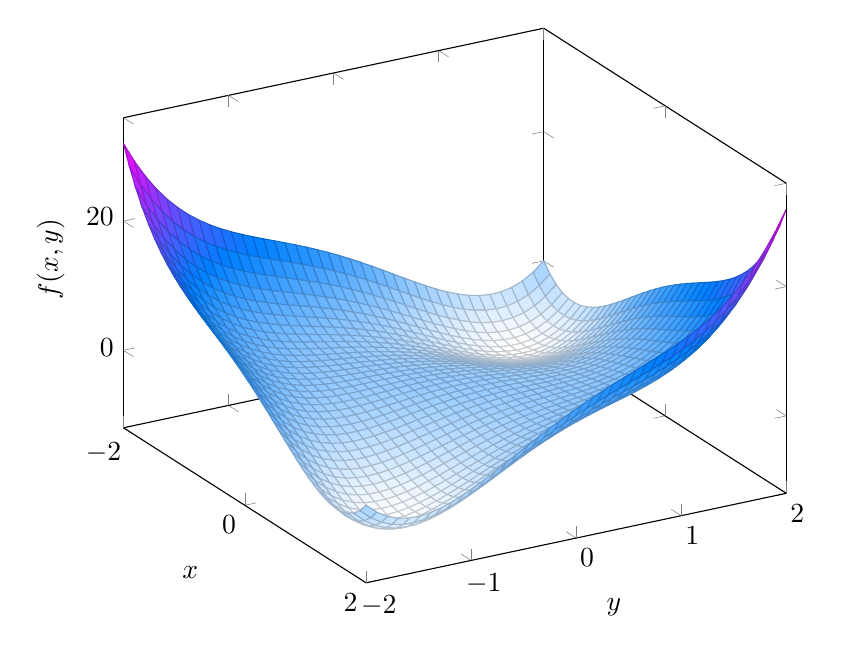
\begin{tikzpicture}
					\begin{axis}[
						width=10cm,
						view={60}{30},
						xlabel={$x$},
						ylabel={$y$},
						zlabel={$f(x,y)$},
						domain=-2:2,
						domain y=-2:2,
						samples=40,
						colormap/cool
						]
						\addplot3[surf] {x^4 + y^4 - 2*(x - y)^2};
					\end{axis}
				\end{tikzpicture}
				%\end{document}
				
			}
	\end{enumerate} 
}